\documentclass[aspectratio=169]{beamer}
\usepackage{enumitem}
\usepackage{tikz}
\usetikzlibrary{shapes, positioning, calc}
\usepackage[export]{adjustbox}
\usepackage{listings}
\usepackage{fontspec}
% \mode<presentation>

\lstset{basicstyle=\ttfamily}
\definecolor{light-gray}{gray}{0.95}
\definecolor{blue}{HTML}{114477}
\definecolor{lightpurple}{HTML}{beaed4}
\definecolor{darkturquoise}{HTML}{00CED1}
\definecolor{sandybrown}{HTML}{F4A460}
\setbeamercolor{title}{fg=blue}
\setbeamercolor{frametitle}{fg=blue}
\setbeamercolor{structure}{fg=blue}

\setbeamertemplate{itemize items}[circle]

\setsansfont{FreeSans}[
    Path=fonts/,
    BoldFont=FreeSansBold,
    ItalicFont=FreeSansOblique,
    BoldItalicFont=FreeSansBoldOblique
]

\title{Genomic analyses of transcription elongation factors\\and intragenic transcription}
\author{James Chuang}
\date{June 19, 2019}

\begin{document}
\begin{frame}
    \titlepage
\end{frame}

\begin{frame}[t]
    \centering
    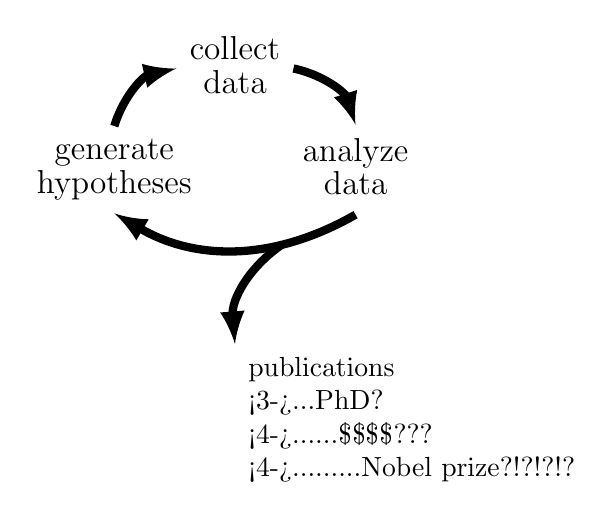
\begin{tikzpicture}[align=center, text depth=.25em, line width=3pt]
        \node [] (hypothesis) {\large generate \\ \large hypotheses};
        \node [] (datacollect) at ($ (hypothesis) + (40:2) $)  {\large collect \\ \large data};
        \node [] (dataanalyze) at ($ (datacollect) + (-40:2) $)  {\large analyze \\ \large data};
        \uncover<2->{\node [align=left, anchor=north west] (publications) at ($ (datacollect) + (-90:3.5) $) {publications \\
                                                                            {\uncover<3->{...PhD?}} \\
                                                                            {\uncover<4->{......\$\$\$\$???}} \\
                                                                            {\uncover<4->{.........Nobel prize?!?!?!?}}
                                                                    };}
        \draw [-latex] (hypothesis.north) to [bend left=30] (datacollect.west);
        \draw [-latex] (datacollect.east) to [bend left=30] (dataanalyze.north);
        \draw [-latex] (dataanalyze.south) to [bend left=30] coordinate[pos=0.3] (midpoint) (hypothesis.south) ;
        \uncover<2->{\draw [-latex] (midpoint) to [bend right=30] (publications.north west);}
    \end{tikzpicture}
\end{frame}

\begin{frame}[t, plain]
    \centerline{
    \begin{tikzpicture}
        \node (rulegraph) {\includegraphics[width=\paperwidth]{figures/rulegraph.pdf}};
        \uncover<2->{\fill [draw=none, fill=white, fill opacity=0.8] (rulegraph.north west) -- (rulegraph.north east) -- (rulegraph.south east) -- (rulegraph.south west) -- (rulegraph.north west) -- cycle;}
        \uncover<2->{\node[] (rule) at (rulegraph.center) {\lstinputlisting[language=Python, backgroundcolor = \color{light-gray}, frame=l, framesep=0.4\textwidth, framerule=0pt, framexbottommargin=1cm]{figures/rule.smk}};}
    \end{tikzpicture}
    }
\end{frame}

\begin{frame}[plain]
    \centerline{\includegraphics[height=\paperheight]{figures/montage.png}}
\end{frame}

\begin{frame}[t,plain]
    \centerline{\includegraphics[width=\paperwidth, trim=0 0 0 0, clip]{figures/zenodo_screenshot.png}}
\end{frame}

\pgfdeclarelayer{backwrapping}
\pgfdeclarelayer{frontwrapping}
\pgfsetlayers{backwrapping,main,frontwrapping}

\tikzset{
        wrapping/.style={
            draw=darkturquoise,
            line cap=round,
            line join=round,
            line width=3pt},
        nucleosome/.style={
            fill=sandybrown!60,
            fill opacity=.9,
            draw=none},
        top cylinder/.style={
            fill=sandybrown!85,
            fill opacity=.9
        }
}

\begin{frame}{transcription}
    \begin{adjustbox}{center}
    \begin{tikzpicture}[scale=0.5]
        \foreach \q [remember=\q as \p] in {1, 2, 4, 5, ..., 9}{
            \begin{scope}[shift={(\q*4,0)}, rotate=30]
                \path [nucleosome]
                    (0.2,1)
                    arc (90:270:0.375 and 1) -- (1,-1)
                    arc (270:90:0.375 and 1) -- cycle;
                \path [top cylinder]
                    (1.375, 0) arc (0:360:0.375 and 1) -- cycle;

                \begin{scope}[shift={(0.25,0)}]
                    \begin{pgfonlayer}{backwrapping}
                    \draw [wrapping]
                        (0.5, -1.125)
                        \foreach \i in {360,355,...,180}{ -- (\i/720+0.375*sin -\i, -1.125*cos \i)}
                        [shift={(-0.5,0)}]
                        (0.5, -1.125)
                        \foreach \i in {360,355,...,200}{ -- (\i/720+0.375*sin -\i, -1.125*cos \i)} coordinate (wrapping-start-\q);
                    \end{pgfonlayer}

                    \begin{pgfonlayer}{frontwrapping}
                    \draw [wrapping]
                        (0, -1.125)
                        \foreach \i in {0,5,...,180}{ -- (\i/720+0.375*sin -\i,-1.125*cos \i)}
                        [shift={(0.5,0)}]
                        (0, -1.125)
                        \foreach \i in {0,5,...,200}{ -- (\i/720+0.375*sin -\i,-1.125*cos \i)} coordinate (wrapping-end-\q);
                    \end{pgfonlayer}
                \end{scope}

                \ifnum\q=1
                    \draw [wrapping] (wrapping-start-\q) to [bend left=15] ++(-1cm,1cm) ;
                \fi
                \ifnum\q>1
                    \draw [wrapping] (wrapping-end-\p) to [bend right=15] coordinate[pos=0.5] (midpoint-\q) (wrapping-start-\q);
                \fi
                % \ifnum\q=2
                %     \draw (midpoint-\q) plot[smooth, tension=.7] coordinates {(1,1)  (1,-1) (-1, 1)};
                % \fi
                \ifnum\q=9
                    \draw [wrapping] (wrapping-end-\q) to [bend right=15] ++(1cm,-1cm);
                \fi
            \end{scope}
        }
    \end{tikzpicture}
    \end{adjustbox}
\end{frame}

\begin{frame}[t,plain]
    \centerline{\includegraphics[width=\paperwidth]{../../structures/elongating_transcription_complex_with_nucleosome.png}}
\end{frame}

\begin{frame}{Spt6 project collaborators}
    \centering
    \begin{description}[align=right, leftmargin=!, labelwidth=5cm, noitemsep]
        \item [Steve Doris] optimized TSS-seq and ChIP-nexus protocols\\generated TSS-seq and ChIP-nexus libraries
        \item [Olga Viktorovskaya] generated MNase-seq libraries
        \item [Magdalena Murawska] generated NET-seq libraries
        \item [Dan Spatt] Northern, Western, and ChIP experiments
    \end{description}
\end{frame}

\begin{frame}{The \textbf{\textit{spt6-1004}} mutant expresses \textbf{intragenic transcripts}}
    \centering
    \begin{columns}
        \begin{column}{0.5\textwidth}
            \includegraphics<1->[width=\textwidth]{figures/presentation/presentation_six_spt6_western.pdf}
        \end{column}
        \begin{column}{0.5\textwidth}
            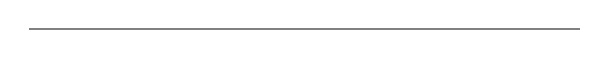
\begin{tikzpicture}
                \draw<2> [line width=1pt, color=gray] (0,0) -- (7,0);
            \end{tikzpicture}
        \end{column}
    \end{columns}
\end{frame}

\begin{frame}[t]
    \begin{tikzpicture}
        \node<1-3>[inner sep=0] (marker) {\includegraphics[width=\textwidth]{figures/presentation/presentation_six_aat_assay_comparison.pdf}};
        \fill<1>[white] (marker.south east) rectangle (-6.55cm, 0.91cm);
        \fill<2>[white] (marker.south east) rectangle (-6.55cm, -1.3cm);
    \end{tikzpicture}
\end{frame}

\begin{frame}[t]
    \begin{tikzpicture}
        \node<1-2>[inner sep=0] (marker) {\includegraphics[width=\textwidth]{figures/presentation/presentation_six_tss_seq_heatmaps.pdf}};
        \fill<1>[white] (marker.south east) rectangle (marker.north);
    \end{tikzpicture}
\end{frame}

\begin{frame}{Downregulation of genic TSSs in \textit{spt6-1004}:}
    \centering
    \begin{columns}
        \begin{column}{0.5\textwidth}
            \includegraphics<1->[width=\textwidth]{figures/presentation/presentation_six_tss_diffexp_summary.pdf}
        \end{column}
        \begin{column}{0.5\textwidth}
            \includegraphics<2>[width=\textwidth]{figures/presentation/presentation_six_tss_expression_levels.pdf}
        \end{column}
    \end{columns}
\end{frame}

\begin{frame}[t]
    \centering
    \includegraphics[width=10.5cm]{figures/presentation/presentation_six_tfiib_heatmap.pdf}
\end{frame}

\begin{frame}{TFIIB binding changes dramatically in \textit{spt6-1004}:}
    \begin{tikzpicture}
        \node<1>[inner sep=0] at (0,0) {\includegraphics[width=15cm]{figures/presentation/presentation_six_tfiib_spreading_swc0001.pdf}};
        \fill<1>[white] (0.3,-0.1) rectangle (3.5, 0.50);
        \node<2>[inner sep=0] at (0,0) {\includegraphics[width=15cm]{figures/presentation/presentation_six_tfiib_spreading_swc0002.pdf}};
    \end{tikzpicture}
\end{frame}

\begin{frame}{new intragenic initiation explains most intragenic transcripts}
    \includegraphics[width=\textwidth]{figures/presentation/presentation_six_tss_v_tfiib.pdf}
\end{frame}

\begin{frame}
    \begin{tikzpicture}
        \node<1>[inner sep=0] at (0,0) {\includegraphics[width=\textwidth]{figures/presentation/presentation_six_mnase_metagene0001.pdf}};
        \fill<1>[white] (-0.7,0.48) rectangle (2.2, 1);
        \node<2>[inner sep=0] at (0,0) {\includegraphics[width=\textwidth]{figures/presentation/presentation_six_mnase_metagene0002.pdf}};
    \end{tikzpicture}
\end{frame}

\begin{frame}
    \centering
    \begin{tikzpicture}
        \node<1-3>[inner sep=0] (marker) at (0,0) {\includegraphics[width=\textwidth]{figures/presentation/presentation_six_intragenic_mnase_metagenes.pdf}};
        \fill<1-3>[white] (2.8,1.15) rectangle (marker.north east);
        \fill<1>[white] (-1.8,-3.825) rectangle (marker.north east);
        \fill<1-2>[white] (2.8,-3.825) rectangle (marker.north east);
    \end{tikzpicture}
\end{frame}

\begin{frame}{GC content}
\end{frame}

\begin{frame}[t]
    \centering
    \includegraphics[width=12cm]{figures/presentation/presentation_six_tss_seqlogos.pdf}
\end{frame}

\begin{frame}
    \centering
    \begin{tikzpicture}
        \node<1>[inner sep=0] at (0,0) {\includegraphics[width=12cm]{figures/presentation/presentation_six_intragenic_tata0001.pdf}};
        % \fill<1>[white] (-0.7,0.48) rectangle (2.2, 1);
        \node<2>[inner sep=0] at (0,0) {\includegraphics[width=12cm]{figures/presentation/presentation_six_intragenic_tata0002.pdf}};
    \end{tikzpicture}
\end{frame}

\begin{frame}{Spt6 summary and model}
\end{frame}

\begin{frame}[t,plain]
    \centerline{\includegraphics[width=\paperwidth]{../../structures/elongating_transcription_complex_with_nucleosome.png}}
\end{frame}

\begin{frame}{Spt5 project collaborators}
    \begin{description}[align=right, leftmargin=!, labelwidth=4cm, noitemsep]
        \item [Ameet Shetty] generated NET-seq, ChIP-seq, RNA-seq,\\TSS-seq, and MNase-seq libraries
    \end{description}
\end{frame}

\begin{frame}{Spt5 depletion system}
    \centering
    \begin{columns}
        \begin{column}{0.45\textwidth}
            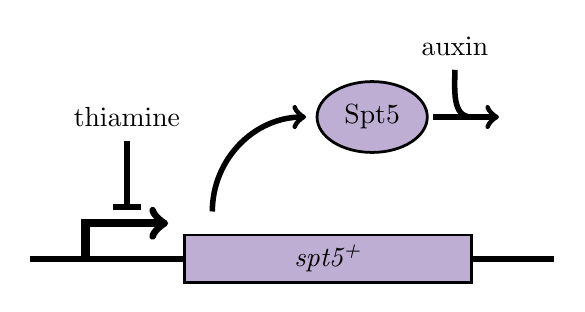
\begin{tikzpicture}[x=7cm, y=3cm]
                \draw [line width=2pt] (0,0.1) -- (0.95,0.1);
                \draw [->, line width=3pt] (0.1,0.1) -- (0.1,0.25) -- (0.25,0.25);
                \draw [line width=2pt] (0.175,0.6) -- (0.175, 0.32);
                \draw [line width=2pt] (0.15, 0.32) -- (0.20, 0.32);
                \node at (0.175, 0.7) {\normalsize thiamine};
                \draw [fill=lightpurple, line width=1pt] (0.28, 0) rectangle (0.8, 0.2);
                \node at (0.54, 0.1) {\normalsize \textit{spt5\textsuperscript{+}}};
                \draw [->, line width=2pt] (0.33, 0.3) to [out=90, in=180] (0.5,0.7);
                \draw [fill=lightpurple, line width=1pt] (0.62, 0.7) circle [x radius=0.1, y radius=0.15];
                \node at (0.62, 0.7) {\normalsize Spt5};
                \draw [->, line width=2pt] (0.73, 0.7) to (0.85, 0.7);
                \node at (0.77, 1) {\normalsize auxin};
                \draw [, line width=2pt] (0.77, 0.9) to [out=270, in=180] (0.80,0.7);
                \node at (0.9, 0.7) {\scalebox{2}{$\varnothing$}};
            \end{tikzpicture}
        \end{column}
        \begin{column}{0.55\textwidth}
            \pause
            \includegraphics[width=\textwidth]{figures/presentation/presentation_five_spt5_depletion.pdf}
        \end{column}
    \end{columns}
\end{frame}

\begin{frame}
    \centering
    \includegraphics[width=12cm]{figures/presentation/presentation_five_netseq_meta.pdf}
\end{frame}

\begin{frame}{wasdas}
    \includegraphics[width=\textwidth]{figures/presentation/presentation_five_rnapii_phosphomark_enrichment.pdf}
\end{frame}

\begin{frame}
    \centering
    \includegraphics[width=12cm]{figures/presentation/presentation_five_rnaseq_metagene.pdf}
\end{frame}

\begin{frame}[t]
    \centering
    \includegraphics[width=10.5cm]{figures/presentation/presentation_five_rnaseq_heatmaps.pdf}
\end{frame}

\begin{frame}[t]
    \includegraphics[width=\textwidth]{figures/presentation/presentation_five_antisense_heatmaps.pdf}
\end{frame}

\begin{frame}[t]
    \includegraphics[width=\textwidth]{figures/presentation/presentation_five_mnase_metagene.pdf}
\end{frame}

\begin{frame}{Spt5 summary and model}
\end{frame}

\begin{frame}{WT intragenic transcription}
\end{frame}

\begin{frame}{project collaborators}
    \centering
\begin{description}[align=right, labelwidth=5cm, noitemsep, leftmargin=!]
    \item [Steve Doris] generated TSS-seq and ChIP-nexus libraries
    \item [Dan Spatt] polyribosome fractionation, competitive growth assays, and Northern blots
    \item [James Warner] Northern blots
\end{description}

\end{frame}

\begin{frame}[t]
    \includegraphics[width=\textwidth]{figures/presentation/presentation_stress_tfiib_ridgelines.pdf}
\end{frame}

\begin{frame}
    \includegraphics[width=\textwidth]{figures/presentation/presentation_stress_tfiib_coverage.pdf}
\end{frame}

\begin{frame}[t]
    \includegraphics[width=\textwidth]{figures/presentation/presentation_stress_promoter_tss_expression.pdf}
\end{frame}

\begin{frame}[t]
    \includegraphics[width=\textwidth]{figures/presentation/presentation_stress_promoter_tss_polyenrichment.pdf}
\end{frame}

\begin{frame}[t]
    \includegraphics[width=\textwidth]{figures/presentation/presentation_stress_dsk2_summary.pdf}
\end{frame}

\begin{frame}
    \begin{columns}
        \begin{column}{0.5\textwidth}
            \includegraphics[width=\textwidth]{figures/presentation/presentation_stress_dsk2_pace_northern.pdf}
        \end{column}
        \begin{column}{0.5\textwidth}
        \end{column}
    \end{columns}
\end{frame}

\begin{frame}
    \includegraphics[width=\textwidth]{figures/presentation/presentation_stress_diamide_fitnesscomp.pdf}
\end{frame}

\end{document}
